\documentclass[10pt,a4paper]{article}
\usepackage[utf8]{inputenc}
\usepackage{graphicx}
\def\Pr{\mathop{\rm Pr}}
%\usepackage[landscape,margin=1cm]{geometry}
\usepackage[english]{babel}
\usepackage{tikz}
\usetikzlibrary{arrows,snakes,backgrounds,shapes.geometric}
\title{Probability and Statistical Inference}
\author{John S Butler}
%\date{July 2019}
\input{cheatsheet-template.tex}


%--------------------------------------------------------------------------------
\begin{document}

%\maketitle
\thispagestyle{empty}
\scriptsize
%\tableofcontents


%\section{Data Type}
\section*{Sorting - Algorithms  (MATH1812)\footnote{\href{https://sites.google.com/dit.ie/math1812/home}{Course Website: https://sites.google.com/dit.ie/math1812/home}}}
%$\subsection*{Cheat Sheet}
\subsubsection*{\href{johnsbutler.netlify.com}{John S Butler} (TU Dublin) }

%%%% EXAMPLE Quick Find

%%% Pesudocode
\section*{Bubble Sort}
\begin{textbox}{Pseudocode}
\begin{subbox}{subbox}{Bubble Sort}
\begin{codebox}{r}{Python Pseudocode}

def Bubble_Sort(a):
n=len(a)
for in range(0,n):
	for j in range(i,n):
		if a[j+1]<a[j]
			a[j]=C
			a[j]=a[j+1]
			a[j+1]=C

    return a
\end{codebox}
\end{subbox}
\end{textbox}
%%% FLOW CHART

\begin{textbox}{Flowchart }
\begin{subbox}{subbox}{Bubble sort}
\begin{center}
    
    
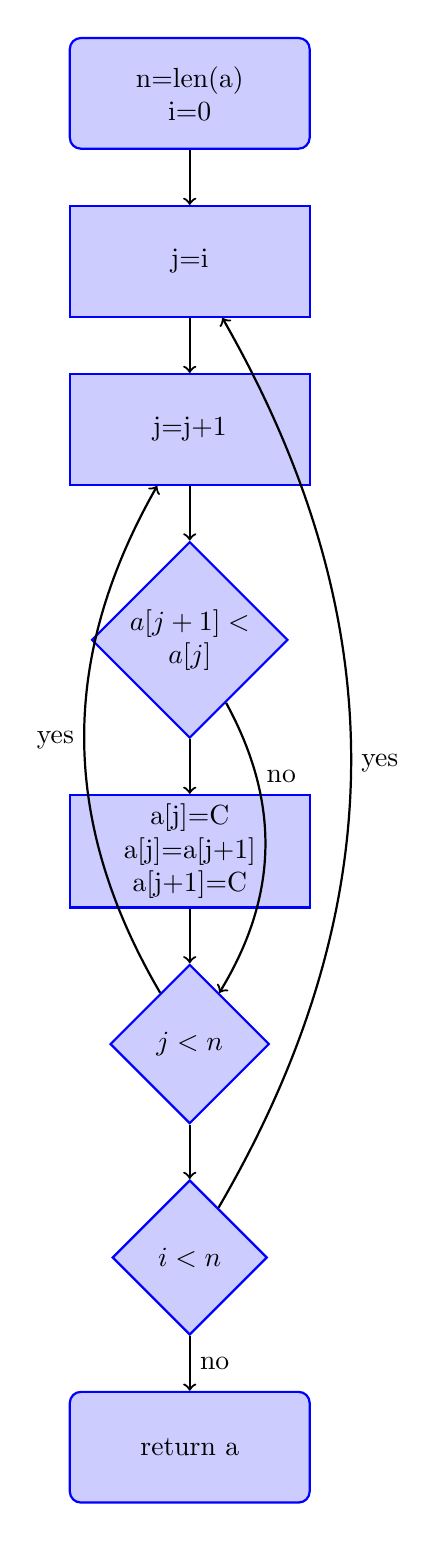
\begin{tikzpicture}[auto]
\tikzstyle{decision} = [diamond, draw=blue, thick, fill=blue!20,
text width=4.5em, text badly centered, inner sep=1pt]

\tikzstyle{block} = [rectangle, draw=blue, thick, fill=blue!20,
text width=8em, text centered, rounded corners, minimum height=4em]
\tikzstyle{block_op} = [rectangle, draw=blue, thick, fill=blue!20,
text width=8em, text centered, minimum height=4em]
\tikzstyle{line} = [draw, thick,->];
\tikzstyle{cloud} = [draw=red, thick, ellipse,fill=red!20, minimum height=2em];
\matrix [column sep=5mm,row sep=7mm]
{
% row 1
 \node [block] (init) {n=len(a)\\i=0}; & \\
% row 2
\node [block_op] (identify) {j=i}; & ;\\
% row 4
\node [block_op] (identify2) {
j=j+1}; & ;\\
\node [decision] (decide_if) {$a[j+1]<a[j]$}; & \\
\node [block_op] (identify_if) {a[j]=C\\
			a[j]=a[j+1]\\
			a[j+1]=C}; & ;\\
\node [decision] (decide) {$j<n$}; & \\
% row 5
\node [decision] (decide2) {$i<n$}; & \\
\node [block] (stop) {return a}; & \\
};
\tikzstyle{every path}=[line]
\path (init) -- (identify);
\path (identify) -- (identify2);
\path  (identify2) --(decide_if);
\path (decide_if) -- (identify_if);
\path (identify_if) -- (decide);
\path (decide_if)  edge [bend left] node[near start,right] {no}  (decide);
\path (decide) -- (decide2);

\path (decide2)  edge [bend right] node[right] {yes}  (identify);

\path (decide)  edge [bend left] node[midway,left] {yes}  (identify2);

\path (decide2) -- node [midway] {no} (stop);

\end{tikzpicture}

\end{center}
\end{subbox}

\end{textbox}

%% SELECTION SORT

\section*{Selection Sort}
\begin{textbox}{Pseudocode}
\begin{subbox}{subbox}{Selection Sort}
\begin{codebox}{r}{Python Pseudocode}

def Selection_Sort(a):
n=len(a)
for i in range(0,n):
	min =i
	c=a[i]
	for j in range(i+1,n):
		if a[j]<a[min]
			min=j 
	
	a[i]=a[min]
	a[min]=c	
    return a
\end{codebox}
\end{subbox}
\end{textbox}
%%% FLOW CHART

\begin{textbox}{Flowchart }
\begin{subbox}{subbox}{Selection sort}
\begin{center}
    
    
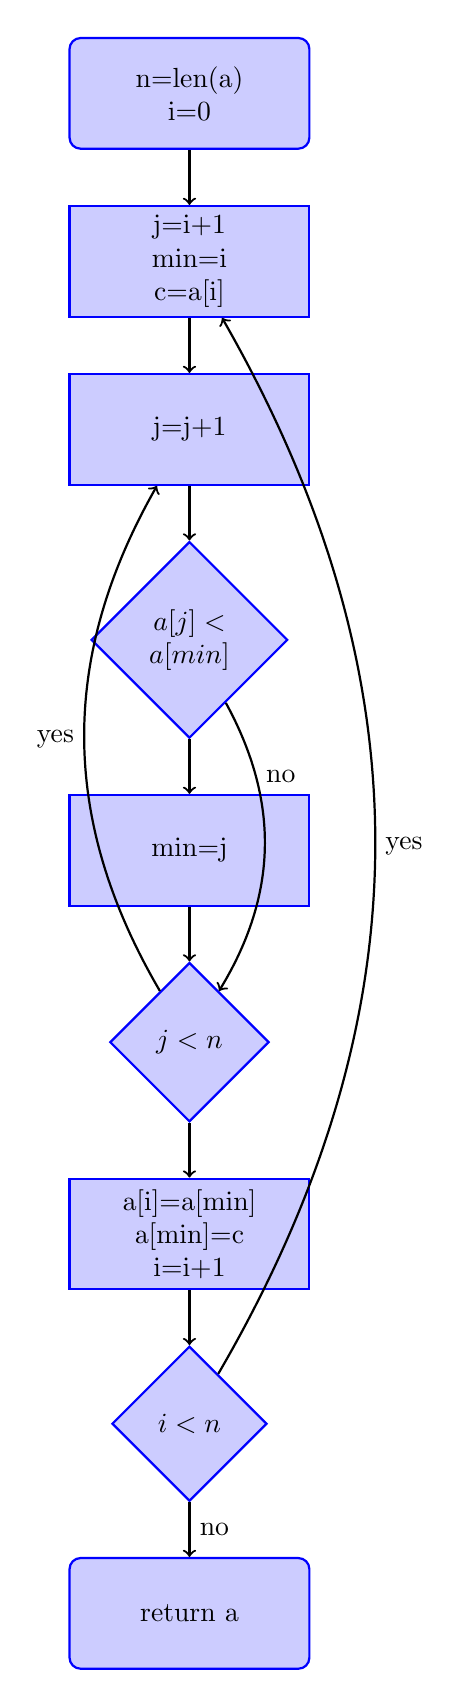
\begin{tikzpicture}[auto]
\tikzstyle{decision} = [diamond, draw=blue, thick, fill=blue!20,
text width=4.5em, text badly centered, inner sep=1pt]

\tikzstyle{block} = [rectangle, draw=blue, thick, fill=blue!20,
text width=8em, text centered, rounded corners, minimum height=4em]
\tikzstyle{block_op} = [rectangle, draw=blue, thick, fill=blue!20,
text width=8em, text centered, minimum height=4em]
\tikzstyle{line} = [draw, thick,->];
\tikzstyle{cloud} = [draw=red, thick, ellipse,fill=red!20, minimum height=2em];
\matrix [column sep=5mm,row sep=7mm]
{
% row 1
 \node [block] (init) {n=len(a)\\i=0}; & \\
% row 2
\node [block_op] (identify) {j=i+1\\ min=i\\c=a[i]}; & ;\\
% row 4
\node [block_op] (identify2) {
j=j+1}; & ;\\
\node [decision] (decide_if) {$a[j]<a[min]$}; & \\
\node [block_op] (identify_if) {min=j}; & ;\\
\node [decision] (decide) {$j<n$}; & \\
% row 5
\node [block_op] (identify3) {
a[i]=a[min]\\
a[min]=c\\
i=i+1}; & ;\\
\node [decision] (decide2) {$i<n$}; & \\
\node [block] (stop) {return a}; & \\
};
\tikzstyle{every path}=[line]
\path (init) -- (identify);
\path (identify) -- (identify2);
\path  (identify2) --(decide_if);
\path (decide_if) -- (identify_if);
\path (identify_if) -- (decide);
%\path (decide_if) node [start] {no} (identify_if);
\path (identify3) -- (decide2);
%\path (decide2) -- (stop);
\path (decide_if)  edge [bend left] node[near start,right] {no}  (decide);
\path (decide) -- (identify3);

\path (decide2)  edge [bend right] node[right] {yes}  (identify);

\path (decide)  edge [bend left] node[midway,left] {yes}  (identify2);

\path (decide2) -- node [midway] {no} (stop);

\end{tikzpicture}

\end{center}
\end{subbox}

\end{textbox}
%% MERGE SORT

\section*{Merge Sort}
\begin{textbox}{Pseudocode}
\begin{subbox}{subbox}{Merge Sort}
\begin{codebox}{r}{Python Pseudocode - Merge }


def merge(array, left_index, right_index, middle):
    left_copy = array[left_index:middle + 1]
    right_copy = array[middle+1:right_index+1]

    left_copy_index = 0
    right_copy_index = 0
    sorted_index = left_index

    while left_copy_index < len(left_copy) and right_copy_index < len(right_copy):

        if left_copy[left_copy_index] <= right_copy[right_copy_index]:
            array[sorted_index] = left_copy[left_copy_index]
            left_copy_index = left_copy_index + 1
        # Opposite from above
        else:
            array[sorted_index] = right_copy[right_copy_index]
            right_copy_index = right_copy_index + 1

       sorted_index = sorted_index + 1

    # Tidy up leftover elements
    while left_copy_index < len(left_copy):
        array[sorted_index] = left_copy[left_copy_index]
        left_copy_index = left_copy_index + 1
        sorted_index = sorted_index + 1

    while right_copy_index < len(right_copy):
        array[sorted_index] = right_copy[right_copy_index]
        right_copy_index = right_copy_index + 1
        sorted_index = sorted_index + 1
        
\end{codebox}
\begin{codebox}{r}{Python Pseudocode - Merge Sort}

def merge_sort(array, left_index, right_index):
    if left_index >= right_index:
        return

    middle = (left_index + right_index)//2
    merge_sort(array, left_index, middle)
    merge_sort(array, middle + 1, right_index)
    merge(array, left_index, right_index, middle)
    
\end{codebox}
\end{subbox}
\end{textbox}
%%% FLOW CHART

\begin{textbox}{Flowchart }
\begin{subbox}{subbox}{Selection sort}
\begin{center}
    
    
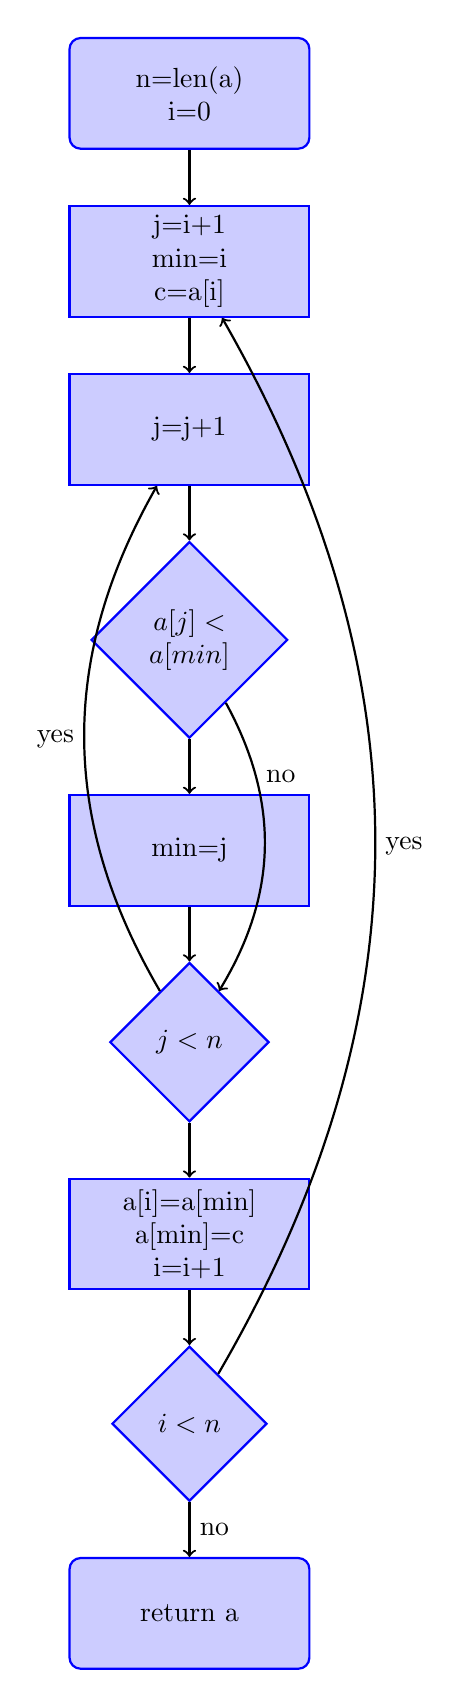
\begin{tikzpicture}[auto]
\tikzstyle{decision} = [diamond, draw=blue, thick, fill=blue!20,
text width=4.5em, text badly centered, inner sep=1pt]

\tikzstyle{block} = [rectangle, draw=blue, thick, fill=blue!20,
text width=8em, text centered, rounded corners, minimum height=4em]
\tikzstyle{block_op} = [rectangle, draw=blue, thick, fill=blue!20,
text width=8em, text centered, minimum height=4em]
\tikzstyle{line} = [draw, thick,->];
\tikzstyle{cloud} = [draw=red, thick, ellipse,fill=red!20, minimum height=2em];
\matrix [column sep=5mm,row sep=7mm]
{
% row 1
 \node [block] (init) {n=len(a)\\i=0}; & \\
% row 2
\node [block_op] (identify) {j=i+1\\ min=i\\c=a[i]}; & ;\\
% row 4
\node [block_op] (identify2) {
j=j+1}; & ;\\
\node [decision] (decide_if) {$a[j]<a[min]$}; & \\
\node [block_op] (identify_if) {min=j}; & ;\\
\node [decision] (decide) {$j<n$}; & \\
% row 5
\node [block_op] (identify3) {
a[i]=a[min]\\
a[min]=c\\
i=i+1}; & ;\\
\node [decision] (decide2) {$i<n$}; & \\
\node [block] (stop) {return a}; & \\
};
\tikzstyle{every path}=[line]
\path (init) -- (identify);
\path (identify) -- (identify2);
\path  (identify2) --(decide_if);
\path (decide_if) -- (identify_if);
\path (identify_if) -- (decide);
%\path (decide_if) node [start] {no} (identify_if);
\path (identify3) -- (decide2);
%\path (decide2) -- (stop);
\path (decide_if)  edge [bend left] node[near start,right] {no}  (decide);
\path (decide) -- (identify3);

\path (decide2)  edge [bend right] node[right] {yes}  (identify);

\path (decide)  edge [bend left] node[midway,left] {yes}  (identify2);

\path (decide2) -- node [midway] {no} (stop);

\end{tikzpicture}

\end{center}
\end{subbox}

\end{textbox}
%% Quick SORT

\section*{Quick Sort}
\begin{textbox}{Pseudocode}
\begin{subbox}{subbox}{Quick Sort}
\begin{codebox}{r}{Python Pseudocode - Partition }

def partition(alist,first,last):
   pivotvalue = alist[first]

   leftmark = first+1
   rightmark = last

   done = False
   while not done:

       while leftmark <= rightmark and alist[leftmark] <= pivotvalue:
           leftmark = leftmark + 1

       while rightmark >= leftmark and alist[rightmark] >=pivotvalue  :
           rightmark = rightmark -1

       if rightmark < leftmark:
           done = True
       else:
           temp = alist[leftmark]
           alist[leftmark] = alist[rightmark]
           alist[rightmark] = temp

   temp = alist[first]
   alist[first] = alist[rightmark]
   alist[rightmark] = temp


   return rightmark

 
\end{codebox}
\begin{codebox}{r}{Python Pseudocode - Quick Sort}

def quickSort(alist):
   quickSortHelper(alist,0,len(alist)-1)

def quickSortHelper(alist,first,last):
   if first<last:

       splitpoint = partition(alist,first,last)

       quickSortHelper(alist,first,splitpoint-1)
       quickSortHelper(alist,splitpoint+1,last)

        
\end{codebox}
\end{subbox}
\end{textbox}
%%% FLOW CHART

\begin{textbox}{Flowchart }
\begin{subbox}{subbox}{Quick sort}
\begin{center}
    
    
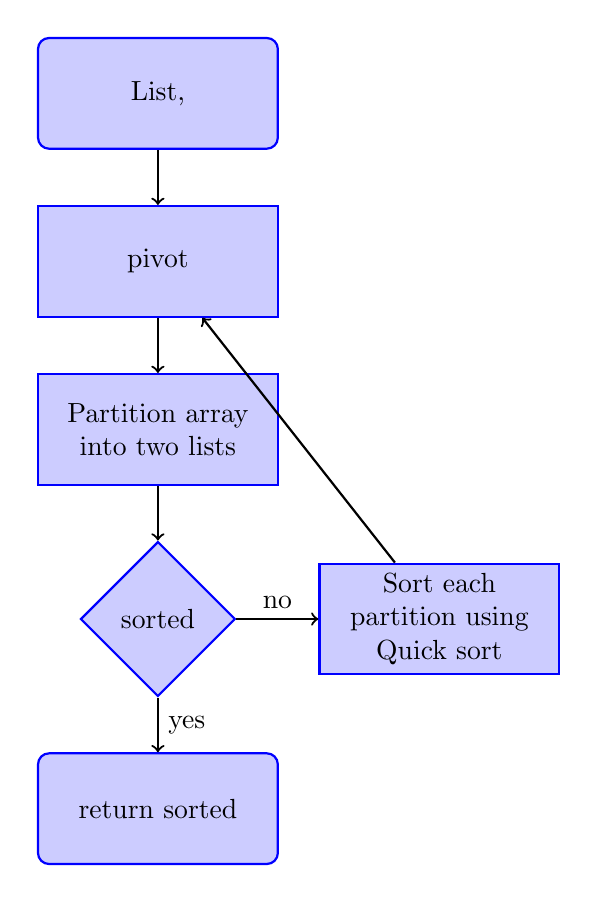
\begin{tikzpicture}[auto]
\tikzstyle{decision} = [diamond, draw=blue, thick, fill=blue!20,
text width=4.5em, text badly centered, inner sep=1pt]

\tikzstyle{block} = [rectangle, draw=blue, thick, fill=blue!20,
text width=8em, text centered, rounded corners, minimum height=4em]
\tikzstyle{block_op} = [rectangle, draw=blue, thick, fill=blue!20,
text width=8em, text centered, minimum height=4em]
\tikzstyle{line} = [draw, thick,->];
\tikzstyle{cloud} = [draw=red, thick, ellipse,fill=red!20, minimum height=2em];
\matrix [column sep=5mm,row sep=7mm]
{
% row 1
 \node [block] (init) {List,}; & \\
% row 2
\node [block_op] (identify) {pivot}; & ;\\
% row 4
\node [block_op] (identify2) {
Partition array into two lists}; & ;\\
\node [decision] (decide_sort) {sorted}; & \node [block_op] (identify3) {
Sort each partition using Quick sort};\\
\node [block] (stop) {return sorted}; & \\
};
\tikzstyle{every path}=[line]
\path (init) -- (identify);
\path (identify) -- (identify2);
\path  (identify2) --(decide_sort);
\path (decide_sort) -- node [midway] {no}  (identify3);
\path (identify3) -- (identify);
\path (decide_sort) -- node [midway] {yes}(stop);


%\path (decide_if) node [start] {no} (identify_if);



\end{tikzpicture}

\end{center}
\end{subbox}

\end{textbox}

\newpage

\begin{textbox}{Flowchart }
\begin{subbox}{subbox}{Merge sort}
\begin{center}
    
    
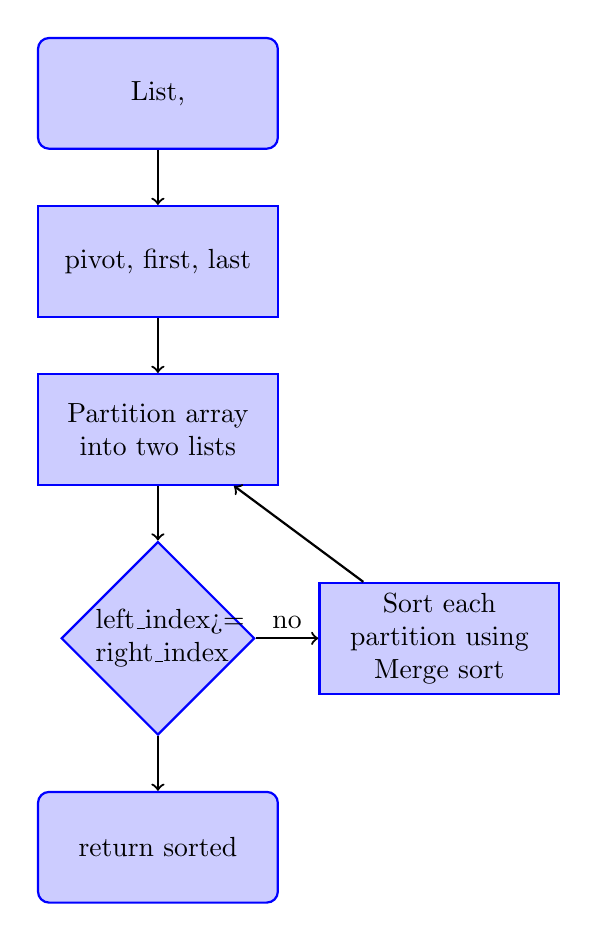
\begin{tikzpicture}[auto]
\tikzstyle{decision} = [diamond, draw=blue, thick, fill=blue!20,
text width=4.5em, text badly centered, inner sep=1pt]

\tikzstyle{block} = [rectangle, draw=blue, thick, fill=blue!20,
text width=8em, text centered, rounded corners, minimum height=4em]
\tikzstyle{block_op} = [rectangle, draw=blue, thick, fill=blue!20,
text width=8em, text centered, minimum height=4em]
\tikzstyle{line} = [draw, thick,->];
\tikzstyle{cloud} = [draw=red, thick, ellipse,fill=red!20, minimum height=2em];
\matrix [column sep=5mm,row sep=7mm]
{
% row 1
 \node [block] (init) {List,}; & \\
% row 2
\node [block_op] (identify) {pivot, first, last}; & ;\\
% row 4
\node [block_op] (identify2) {
Partition array into two lists}; & ;\\
\node [decision] (decide_sort) {left\_index>= right\_index}; & \node [block_op] (identify3) {
Sort each partition using Merge sort};\\
\node [block] (stop) {return sorted}; & \\
};
\tikzstyle{every path}=[line]
\path (init) -- (identify);
\path (identify) -- (identify2);
\path  (identify2) --(decide_sort);
\path (decide_sort) -- node [midway] {no}  (identify3);
\path (identify3) -- (identify2);
\path (decide_sort) -- (stop);


%\path (decide_if) node [start] {no} (identify_if);



\end{tikzpicture}

\end{center}
\end{subbox}

\end{textbox}
\end{document}
